\documentclass[a4paper,10pt]{article}
\usepackage[utf8]{inputenc}
\usepackage[french]{babel}
\usepackage[T1]{fontenc}
\usepackage{lmodern}
\usepackage{graphicx}
\usepackage{listings}
\usepackage{xcolor}
\usepackage{textcomp}
\setlength{\textwidth}{16cm}
\setlength{\marginparwidth}{0cm}
\setlength{\oddsidemargin}{0cm}
\setlength{\headheight}{0cm}
\setlength{\topmargin}{0cm}
\setlength{\headsep}{0cm}
\setlength{\textheight}{25cm}
\setlength{\footskip}{0cm}
\setlength{\marginparsep}{0cm}
\lstset{basicstyle=\small\ttfamily,breaklines=true}
\usepackage{listings}
\usepackage{xcolor}
\usepackage{textcomp}
\lstset{language=c++,basicstyle=\small\ttfamily,keywordstyle=\color{blue}\ttfamily,stringstyle=\color{red}\ttfamily,commentstyle=\color{green}\ttfamily,breaklines=true}


%opening
\title{Compte Rendu \\ NACHOS}
\author{BARTHELEMY Romain, EUDES Robin, MORISON Jack, ROSSI Ombeline}


\begin{document}
\maketitle
\tableofcontents
\newpage
\section{Introduction}
Ce projet a été réalisé dans le cadre de notre 4ème année d'étude à Polytech, avec la spécialisation ``systèmes et réseaux''.
En réalisant ce projet, nous avons pu mettre en pratique l'ensemble des connaissances engrangées au cours de nos parcours et ainsi
comprendre les concepts entrant en jeu lors de la réalisation d'un système d'exploitation.
\vspace{0.5cm}

Dans un premier temps, nous allons nous intéresser au fonctionnement d'un appel système, comment le système les détecte, les gère.
Dans une seconde partie, nous étudierons le multithreading, et de façon plus générale la gestion des threads par NachOS.

\newpage
\section{Étape 2 : Etude d'un syscall}
\subsection{Entrées-sorties asynchrones}
Une version élémentaire de gestion des entrées-sorties nous est fournie par NachOS, au travers de la classe \textit{Console}. Le code fourni
effectue une  gestion asynchrone des entrées-sorties. Nous devons donc gérer la synchronisation grâce à deux sémaphores (pour gérer l'écriture et la lecture)
ainsi que deux handlers. Ceux-ci libèreront le sémaphore et nous informeront de la fin de l'opération de lecture/écriture. Ainsi, la synchronisation est assurée
par ce mécanisme.

Voici un extrait de code permettant cette gestion des entrées/sorties. Si le caractère est EOF, la machine s'arrête.
\begin{lstlisting}[frame=single]
void ConsoleTest (char *in, char *out){
    char ch;
    console = new Console (in, out, ReadAvail, WriteDone, 0);
    readAvail = new Semaphore ("read avail", 0);
    writeDone = new Semaphore ("write done", 0);

    for (;;) {
	  readAvail->P (); // wait for character to arrive
	  ch = console->GetChar ();
	  
	  #ifdef CHANGED
	  if(ch!='\n' && ch!=EOF){
		  console->PutChar ('<');
		  writeDone->P ();
	  }
	  #endif
	  
	  // Original code
	  #ifndef CHANGED 
	  console->PutChar (ch);
	  writeDone->P (); // wait for write to finish
	  if (ch == 'q')
		  return;
	  #else
	  
	  // Now, we prefer to exit on EOF,
	  // only if it's at the beginning of a new line.
	  if(ch!=EOF){
		  console->PutChar (ch);
		  writeDone->P ();
		  if(ch!='\n'){
			  console->PutChar ('>');
			  writeDone->P ();
		  }
	  }
	  else{
		return;
	  }
	  if (ch=='\0'){ // EOT
		  return;
	  }
      #endif
      }
}
\end{lstlisting}
\newpage
\subsection{Entrées-sorties synchrones}
Nous devons maintenant créer une classe \textit{SynchConsole} afin de réaliser les opérations de synchronisation d'entrées/sorties automatiquement :
\begin{lstlisting}[frame=single]

static Semaphore *readAvail;
static Semaphore *writeDone;
static Semaphore *SemPutChar;
static Semaphore *SemGetChar;
static Semaphore *SemPutString;
static Semaphore *SemGetString;

static void ReadAvail(int arg) { readAvail->V(); }
static void WriteDone(int arg) { writeDone->V(); }

SynchConsole::SynchConsole(char *readFile, char *writeFile){
	readAvail = new Semaphore("read avail", 0);
	writeDone = new Semaphore("write done", 0);
	console = new Console (readFile, writeFile, ReadAvail, WriteDone, 0);

	SemPutChar = new Semaphore("PutChar", 1);
	SemGetChar = new Semaphore("GetChar", 1);
	SemPutString = new Semaphore("PutString", 1);
	SemGetString = new Semaphore("GetString", 1);
}

SynchConsole::~SynchConsole(){
	delete console;
	delete writeDone;
	delete readAvail;
}

void SynchConsole::SynchPutChar(const char ch){
	SemPutChar->P();
	console->PutChar (ch);
	writeDone->P ();
	SemPutChar->V();
}

char SynchConsole::SynchGetChar(){
	SemGetChar->P();
	char ch;
	readAvail->P ();
	ch = console->GetChar ();
	SemGetChar->V();
	return ch;
}
\end{lstlisting}
\newpage
Le test de ces méthodes est réalisé dans \textit{progtest.cc} par la fonction \textit{SynchConsoleTest}.
\begin{lstlisting}[frame=single]
 void SynchConsoleTest (char *in, char *out){
	char ch;
	SynchConsole *synchconsoletest = new SynchConsole(in, out);

	while ((ch = synchconsoletest->SynchGetChar()) != EOF){
		if(ch!='\n'){
			synchconsoletest->SynchPutChar('<');
			synchconsoletest->SynchPutChar(ch);
			synchconsoletest->SynchPutChar('>');
		}
		else{
			synchconsoletest->SynchPutChar(ch);
		}
	}
	fprintf(stderr, "Solaris: EOF detected in SynchConsole!\n");
}
\end{lstlisting}
\textit{Note : Chaque caractère est par ailleurs encadré par < >}

Le fichier \textit{main.cc} est modifié pour prendre en compte l'option -sc qui permettra l'éxecution de la console synchrone.
Initialement, la création de la console était effectuée dans \textit{system.cc , fonction Initialize}, mais suite à des erreurs
rencontrées dans les phases de test, l'instanciation de SynchConsole a été déplacée dans le main.
\begin{lstlisting}[frame=single]
#ifdef CHANGED
...
else if (!strcmp (*argv, "-sc")){
	if (argc == 1)
	    SynchConsoleTest (NULL, NULL);
	else
	  {
	      ASSERT (argc > 2);
	      SynchConsoleTest (*(argv + 1), *(argv + 2));
	      argCount = 3;
	  }
	interrupt->Halt ();
}
#endif // CHANGED
\end{lstlisting}
En conséquence, la fonction \textit{Cleanup() (system.cc)} est modifiée, pour supprimer cette nouvelle console lors de l'arrêt de NachOS.
\begin{lstlisting}[frame=single]
#ifdef CHANGED
    delete synchconsole;
#endif //CHANGED
\end{lstlisting}
\newpage
\subsection{Création du syscall Putchar}
Pour réaliser cet appel système, nous modifions \textit{syscall.h}, afin d'y ajouter une constante associée au syscall putchar.
Cette constante indiquera au handler la nature de l'exception (  \textit{exception.cc, fonction ExceptionHandler} ).
\begin{lstlisting}[frame=single]
 #define SC_PutChar		11
\end{lstlisting}
Le syscall est ensuite défini dans \textit{start.S} (en assembleur), en nous inspirant des syscall existants.

\begin{lstlisting}[frame=single]
	.globl PutChar
	.ent	PutChar
PutChar:
	addiu $2,$0,SC_PutChar
	syscall
	j	$31
	.end PutChar
\end{lstlisting}
Le syscall \textit{PutChar} défini, il nous reste à mettre en place le handler qui se chargera de la gestion
des exceptions relatives à PutChar (\textit{exception.cc, fonction ExceptionHandler}) :

\begin{lstlisting}[frame=single]
if (which == SyscallException){
	switch(type){
		case SC_Halt:{
			DEBUG ('a', "Shutdown, initiated by user program.\n");
			interrupt->Halt ();
			break;
		}
		case SC_PutChar:{
			int c = machine->ReadRegister (4);
			synchconsole->SynchPutChar((char)c);
			break;
		}
		default:{
			printf ("Unexpected user mode exception %d %d\n", which, type);
			ASSERT (FALSE);
		}
	}
}
\end{lstlisting}
\newpage
\subsection{La manipulation de chaine de caractères}
La manipulation des string nous permet d'étudier les spécificités de la simulation d'un système d'exploitation par NachOS.
En effet, nous devons jongler entre 2 espaces mémoire : l'espace MIPS (NachOS) et l'espace Linux.
\begin{lstlisting}[frame=single]
// Used for SynchPutString 
// get string from mips memory space, put it in linux memory space
void copyStringFromMachine( int from, char *to, unsigned size){
	unsigned int i;
	int tmp;
	for(i=0;i<size;i++){
		if(machine->ReadMem(from+i,1,&tmp))
		to[i]=tmp;
	}
	if(tmp!='\0'){
		to[size-1]='\0';
	}
}
// Used for SynchGetString
// get string from linux memory space, put it to mips memory space
void copyStringToMachine( char *from, int to, unsigned size){
	unsigned int i;
	int tmp;
	for(i=0;i<size-1;i++){
		tmp=from[i];
		machine->WriteMem(to+i,1,tmp);
	}
	tmp='\0';
	machine->WriteMem(to+i,1,tmp);
}
\end{lstlisting}

Nous devons ensuite ajouter les syscall associés SynchPutString et SynchGetString (\textit{start.S}) :
\begin{lstlisting}[frame=single]
 SynchPutString:
	addiu $2,$0,SC_SynchPutString
	syscall
	j	$31
	.end SynchPutString

	.globl SynchGetChar
	.ent	SynchGetChar
SynchGetString:
	addiu $2,$0,SC_SynchGetString
	syscall
	j	$31
	.end SynchGetString

	.globl SynchPutInt
	.ent	SynchPutInt
\end{lstlisting}
\newpage
Et mettre en place les handlers associés, comme pour les précédents appels système. (\textit{exception.cc, fonction ExceptionHandler}) :
\begin{lstlisting}[frame=single]
case SC_SynchPutString:{
	char *buffer=new char[MAX_STRING_SIZE];
	int s = machine->ReadRegister (4);
	copyStringFromMachine(s, buffer, MAX_STRING_SIZE);
	synchconsole->SynchPutString(buffer);
	delete buffer;
	break;
}
case SC_SynchGetString:{
	char *buffer=new char[MAX_STRING_SIZE];
	int s = machine->ReadRegister (4);
	int size = machine->ReadRegister (5);
	synchconsole->SynchGetString(buffer,size);
	copyStringToMachine(buffer, s, size);
	delete buffer;
	break;
}
\end{lstlisting}
\textit{Note : MAX\_STRING\_SIZE , SC\_SynchPutString, SC\_SynchGetString sont définis dans system.h }
\newpage

Enfin, les fonctions SynchPutString et SynchGetString sont définies dans \textit{SynchConsole.cc}, elles seront appelé
par le handler associé.

\begin{lstlisting}[frame=single]
void SynchConsole::SynchPutString(const char s[]){
SemPutString->P();
int i;
for (i=0;i<MAX_STRING_SIZE && s[i]!='\0';i++){
	if (s[i]=='\0')
	return;
	synchconsole->SynchPutChar ((char)s[i]);
}
SemPutString->V();
}

void SynchConsole::SynchGetString(char *s, int n){
SemGetString->P();
char c;
int i;

c = synchconsole->SynchGetChar ();
if(c==EOF || c=='\n'){
	s[0]='\0';
	SemGetString->V();
	return;
}
else
	s[0] = c;
for (i=1;i<n;i++){
	c = synchconsole->SynchGetChar ();
	if(c==EOF && s[i-1]=='\n')
		break;
	else{
		if(c==EOF)
			i--;
		else
			s[i] = c;
	}
}
s[i]='\0';
SemGetString->V();
}
\end{lstlisting}
La méthode SynchGetString est un peu plus complexe que SynchPutString car nous devons maintenir un comportement :
Si EOF est vu en début de ligne, on termine la console, sinon ce dernier est ignoré (comme dans un système Linux).
\newpage
\subsection{Déroulement global d'un syscall}
Par cet exercice autour d'une console synchrone, nous comprenons désormais le mécanisme d'appel système.
\begin{figure}[h]
  \begin{center}
    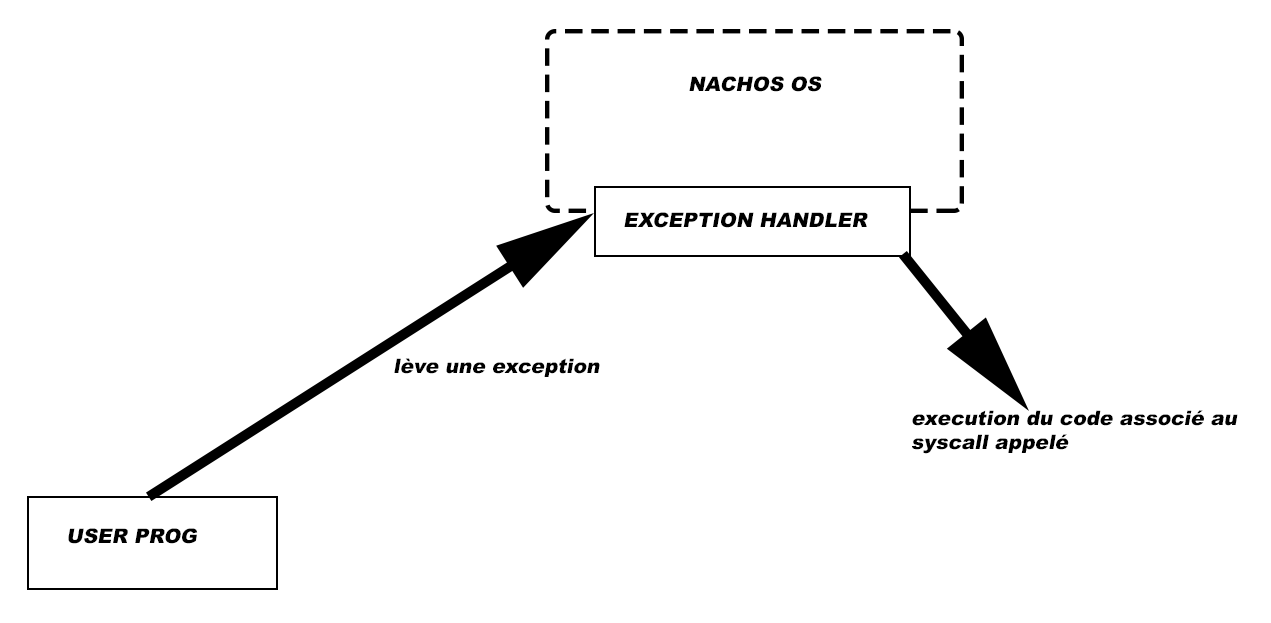
\includegraphics[scale=0.3]{./nachos_syscall.png}
   \caption{\label{syscall} Mécanique simplifiée d'un syscall}
  \end{center}
\end{figure}
\newpage
\begin{figure}[h]
\begin{center}
    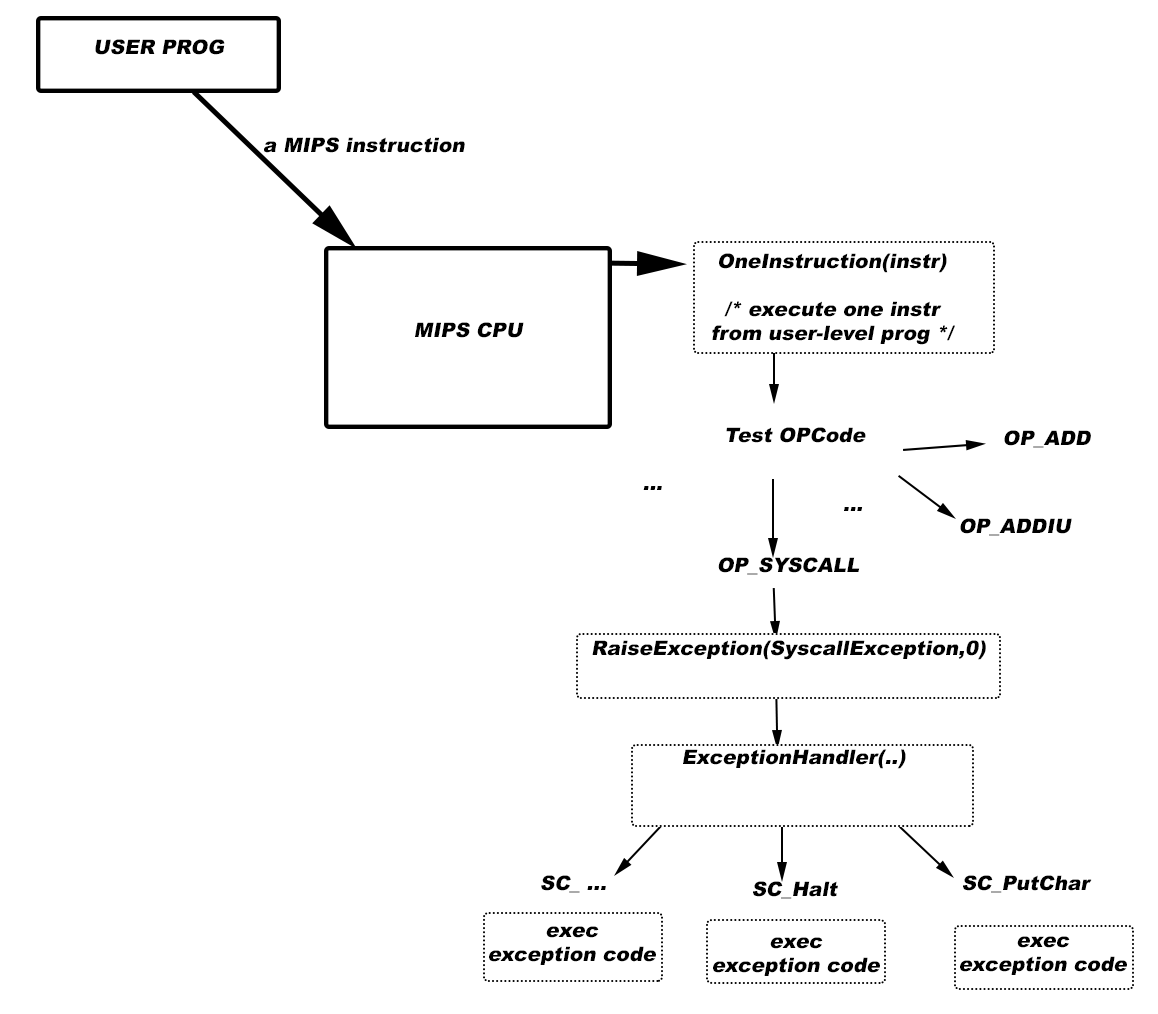
\includegraphics[scale=0.39]{./nachos_syscall_details.png}
   \caption{\label{syscall_det} Mécanique détaillée d'un syscall}
  \end{center}
\end{figure}


On retrouve par ailleurs les mécaniques d'intéruptions vu en RICM3, dans le code de la fonction RaiseException (machine.cc).
On passe en Kernel Mode pour la gestion de l'exception, puis on revient en User Mode.


\newpage
\section{Étape 3 : Multithreading}
Nous nous intéréssons désormais aux threads. Nous souhaitons au terme de cette étape pouvoir éxecuter des programmes utilisateurs multi-thread
sur NachOS. Nous allons d'abord comprendre le fonctionnement d'un thread NachOS, afin de pouvoir ensuite utiliser cette mécanique pour nos threads utilisateur.

\subsection{Thread Nachos}
Les threads NachOS sont créés et initialisés dans la méthode \textit{Thread()} dans le fichier \textit{thread.cc}.
\begin{lstlisting}[frame=single]
 Thread::Thread (const char *threadName){
    name = threadName;
    stackTop = NULL;
    stack = NULL;
    status = JUST_CREATED;

#ifdef USER_PROGRAM
#ifdef CHANGED
    dependance=-1;
#endif //CHANGED

    space = NULL;

    for (int r=NumGPRegs; r<NumTotalRegs; r++)
      userRegisters[r] = 0;
#endif
}
\end{lstlisting}
La pile est initialisée. On positionne un entier ``dépendance'' à -1 (aucune dépendance vers un autre thread). Cette variable ajoutée nous sera utile par la suite,
pour ajouter une dépendance du thread courant vers un autre thread. Ensuite, l'espace mémoire du thread, (code exécuté par le thread) est initialisé à NULL. Enfin,
les registres sont initialisés. À ce niveau, le thread a le statut \textit{JUST\_CREATED}, il n'est pas encore prêt à être lancé.

\vspace{0.5cm}

Pour rendre un thread exécutable, un appel à la méthode \textit{Fork} doit être effectué. Cette méthode prend en paramètre un pointeur vers le programme à charger en mémoire, et
les paramètres de la fonction (pointeur vers une structure contenant les arguments). Le thread ``forké'' partage le même espace mémoire que les autres thread du processus.
Son statut est mis à jour ( \textit{READY} ). Enfin, il est placé dans la ReadyQueue , le thread a un programme à exécuter.

\newpage

Lors de la mise en place de l'espace d'adressage, le code qui sera exécuté par le thread est placé dans un objet \textit{NoffHeader}.

\begin{figure}[h]
  \begin{center}
    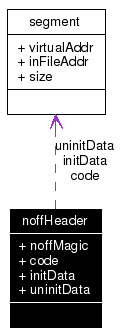
\includegraphics[scale=0.4]{./structnoff.png}
   \caption{\label{structnoff} Structure NoffHeader}
  \end{center}
\end{figure}

NoffMagic est un entier identifiant l'objet contenant le code à éxecuter comme étant de type NachOS.
La documentation nous apprend par ailleurs que le format d'object NachOS est une simplification du format d'oject UNIX.
Cet objet contient les segments code ( code exécutable ) et initdata (données initiales), entre autres.
Ces données sont contenues dans un espace d'adressage propre au thread dont la taille est de 4*1024 bits (StackSize défini dans \textit{thread.h}).
Par ailleurs, en lisant les commentaires, nous apprenons que nous allouons, dans cette simulation, un même espace (thread's private execution stack),
indépendament du code exécuté par le thread. StackSize doit donc être de taille suffisante, pour nous éviter des erreurs diverses...
\vspace{0.5cm}

Le système divise cet espace en pages, puis il effectue la correspondance entre les adresses physiques et les adresses virtuelles.
En observant le code fourni dans \textit{addrspace.cc}, nous pouvons comprendre le fonctionnement des fonctions \textit{saveUserState} et \textit{restoreUserState}.
La fonction \textit{saveUserState} sauvegarde les registres qui sont utilisés par le thread. Ces données sont sauvegardées dans le tableau userRegisters,
propre à chaque thread. La fonction \textit{restoreUserState} effectue l'opération inverse, en restaurant les registres du thread.
Les données sont ensuite chargé en mémoire, en utilisant la table des pages créée précédement. Ces dernières étapes sont réalisées dans le constructeur d'AddrSpace.
\vspace{0.5cm}

À ce niveau, les pages virtuelles sont des pages physiques, l'adressage virtuel sera réalisé dans l'étape 4.

\newpage
\subsection{Thread Utilisateur}
Cette mécanique autour des threads est utilisée afin de supporter chaque thread utilisateur par un thread NachOS.
Nous étudions maintenant \textit{StartProcess(..) , progtest.cc }. Après avoir chargé le programme à exécuter en mémoire,
les registres sont initialisés(\textit{PCReg, NextPCReg, StackReg}, et les autres registres de NachOS) puis le programme est lancé, grâce à la méthode \textit{Run()}.
\subsubsection{Syscall UserThreadCreate}
On souhaite maintenant qu’un programme utilisateur puisse créer des threads au niveau utilisateur,
c’est-à-dire effectuer un appel système \textit{int UserThreadCreate(void f(void *arg), void *arg)}.
Nous réutilisons donc les mécaniques de l'étape précédante, pour mettre en place le syscall voulu.

Lors de l'appel système UserThreadCreate, nous appelons \textit{do\_UserThreadCreate}.
Cette première fonction de manipulation des threads utilisateurs est définie dans \textit{userthread.cc}.
Pour l'instant, nous nous intéréssons uniquement aux opérations liéé à la création d'un thread utilisateur.
Certaines mécaniques ont du être ajouté pour assurer la cohérence de la page table et le bon fonctionnement d'une dépendance
entre deux threads.

\begin{lstlisting}[frame=single]
int do_UserThreadCreate(int f, int arg){

if(!currentThread->space->CheckFreeStack()){
  printf("Error: Stack already full\n");
  return -1;
}

Thread *t = new Thread("UserThread");

if(t==NULL){
  printf("Error: Thread non created\n");
  return -1;
}

// En cas de user_join, mutex autour de son init
//  -> eviter une dep vers un thread pas encore init.
CheckThreadExistence->P();

argThread *argt = new argThread;
argt->func = f;
argt->argv = arg;

t->Fork(StartUserThread,(int)argt);

// Afin que l'alloc dans la stack soit secure
await->P();

// Prend le sem, si un autre t a une dep sur lui -> en attente sur sem.
currentThread->space->TabSemJoin[t->initStackReg]->P();

// set id thread into result reg, useful for join fct...
machine->WriteRegister(2, t->initStackReg);

CheckThreadExistence->V();

currentThread->Yield();

return 0;
}
\end{lstlisting}
\newpage
Le thread user créé, nous devons le lancer. Cette opération est réalisée par la fonction \textit{StartUserThread}.
Le prototype de la fonction nous impose un unique paramètre. Nous devons passer les paramètres suivant : le poiteur vers la fonction et un pointeur vers les paramètres
de la fonction. Nous avons créé une structure regroupant ces paramètres. Nous passerons un pointeur vers cette structure en paramètre à \textit{StartUserThread}.
\begin{lstlisting}[frame=single]
 typedef struct{
		int func;
		int argv;
	}argThread;
\end{lstlisting}

Toute les instructions exécutées après le Fork sont réalisées par le ``père'' et ont pour but d'assurer
le bon fonctionnement d'une dépendance vers le thread créé par le Fork.

\subsubsection{Lancement du thread}

\begin{lstlisting}[frame=single]
 static void StartUserThread(int f){
argThread *argt = (argThread *) f;

//Save old registers
currentThread->space->SaveState();
//Clean registers
currentThread->space->InitRegisters();

// On place PC sur notre fonction
machine->WriteRegister (PCReg,argt->func);
machine->WriteRegister (NextPCReg,(argt->func)+4);
// argument de notre fct
machine->WriteRegister (4,argt->argv);
// init page , retourne id ds bitmap
int alloc = currentThread->space->AllocStack();
// maj sommet pile
machine->WriteRegister (StackReg,currentThread->space->StackValue(alloc));
//save bitmap page id thread (necesaire pour liberer l'espace ensuite )
currentThread->initStackReg=alloc;

// Alloc dans la stack terminee
//(  important pour que join fonctionne bien)
// on controle pas quand l'OS commute...
await->V();

machine->Run();
}
\end{lstlisting}

Voici comment est réalisé l'allocation de la mémoire dans la pile pour notre thread:
\begin{lstlisting}[frame=single]
 int AddrSpace::AllocStack () {
	if((stack->NumClear())<=0){
		printf("Stack overflow\n");
		return -1;
	}
	SemThread->P();	
	int tmp = stack->Find();
	stack->Mark(tmp);
	nbThreads++;
	SemThread->V();
	return tmp;
}
\end{lstlisting}

On recherche la première page libre, on la marque comme ``occupée''. Un compteur du nombre de thread est incrémenté.
Ce dernier empeche le syscall Halt d'arrêter NachOS tant qu'un thread utilisateur existe ( et n'a pas terminé ).
\newpage
\subsubsection{Syscall UserThreadExit}
Le thread utilisateur lancé, nous devons maintenant nous intéresser à son arrêt.
Un nouvel appel système \textit{UserThreadExit} est créé, ce dernier fait appel à la fonction suivante :

\begin{lstlisting}[frame=single]
 int do_UserThreadExit(){

 // free bitmap page
 currentThread->space->FreeStack(currentThread->initStackReg);
 
 currentThread->space->TabSemJoin[currentThread->initStackReg]->V();
 
 if(currentThread->dependance!=-1)
  currentThread->space->TabSemJoin[currentThread->dependance]->V();
 
 currentThread->Finish();
 
 return 0;
}
\end{lstlisting}
\newpage
\subsubsection{Syscall UserThreadJoin}
Enfin, nous réalisons un dernier appel système, UserThreadJoin afin de forcer un thread à attendre la terminaison d'un thread (autre que lui même ou le thread principal).
Pour mettre en place ce fonction, nous avons du mettre en place un système de sémaphore dans les précédantes fonctions.

Lors de la création du thread ( \textit{do\_UserThreadCreate(...)}) , nous effectuons plusieurs manipulations  après le Fork. Nous prenons d'abord un sémaphore \textit{await}.
Il sera libéré à la fin de \textit{StartUserThread} juste avant l'appel à \textit{Run()}. Ce sémaphore assure la cohérence de la bitmap. En effet, si un autre thread veut effectuer
un join vers un thread créé plus tôt, ce dernier doit avoir terminé son allocation dans la pile. Si le thread principal veut créer un autre fils, il devra donc attendre que 
l'allocation du premier soit terminé. Nous prenons ensuite un second sémaphore \textit{TabSemJoin[t->initStackReg]}.
Si un thread X fait un join vers ce thread, il devra attendre que le semaphore soit libéré par notre thread lors de l'appel à do\_UserThreadExit() pour prendre le sémaphore
(on prend ce semaphore dans UserThreadJoin(..) ). Ainsi, on force l'ordre d'exécution ( la dépendance voulue !) , en forcant une attente du thread X sur le semaphore 
corespondant au thread dont on veut dépendre.

Lors de la terminaison du thread \textit{do\_UserThreadExit()}, le thread libère le sémaphore associé à son thread.
Ainsi, il débloque d'éventuels thread en attente sur ce sémaphore, des thread qui avaient donc une dépendance vers lui.
Si il avait lui même une dépendance, et qu'il est dans cette méthode, alors il doit libérer le sémaphore vers cette dépendance,
permettant donc à d'autres threads en attente sur cette dernière de s'exécuter. Par cette mécanique de sémaphore, nous nous assurons d'avoir autant de P() que de V()
sur les différents sémaphores, nous évitons donc tout deadlock.
 
\begin{lstlisting}[frame=single]
 int UserThreadJoin(int t){
if(currentThread->dependance!=-1){
  printf("Le thread possede deja une dependance\n");
  return -1;
}
if(currentThread->initStackReg==t || t==0){
  printf("Tentative de dependance vers un thread invalide\n");
  return -1;
}
CheckThreadExistence->P();

if(!currentThread->space->Test(t)){
  printf("Tentative de dependance vers un thread non existant\n");
  CheckThreadExistence->V();
  return -1;
}

CheckThreadExistence->V();

currentThread->dependance=t;
currentThread->space->TabSemJoin[t]->P();
return 0;
}
\end{lstlisting}
\newpage
\subsection{Test du multithreading utilisateur}

\begin{lstlisting}[frame=single]
 #include "syscall.h"

void thread(int *i){
	if(*i!=-1){
		UserThreadJoin(*i);
		SynchPutString("Thread ");
		SynchPutInt(*i);
		PutChar('\n');
	}
	else{
		SynchPutString("Thread initial\n");
		int a=1001;
		int j;	
		//Calcul sale pour "ralentir" le premier thread
		for(j=0;j<1000;j++){
			if(a%2){
				a=a*2;
			}
			else{
				a=a/2;
			}
		}
	}
	UserThreadExit();
}

int main(){
	int param=-1;
	int t1 = UserThreadCreate((void (*)(void *))thread,(void *)(&param));
	int t2 = UserThreadCreate((void (*)(void *))thread,(void *)(&t1));
	UserThreadJoin(t2);
	SynchPutString("Main program terminated\n");
	Halt();
}

// Trace d'execution
./nachos-step2 -x makemultithreads
Thread initial
Thread 1
Main program terminated
Machine halting!
\end{lstlisting}
\newpage
\subsection{Déroulement d'une exécution avec dépendance entre 2 threads}
\begin{figure}[h]
  \begin{center}
    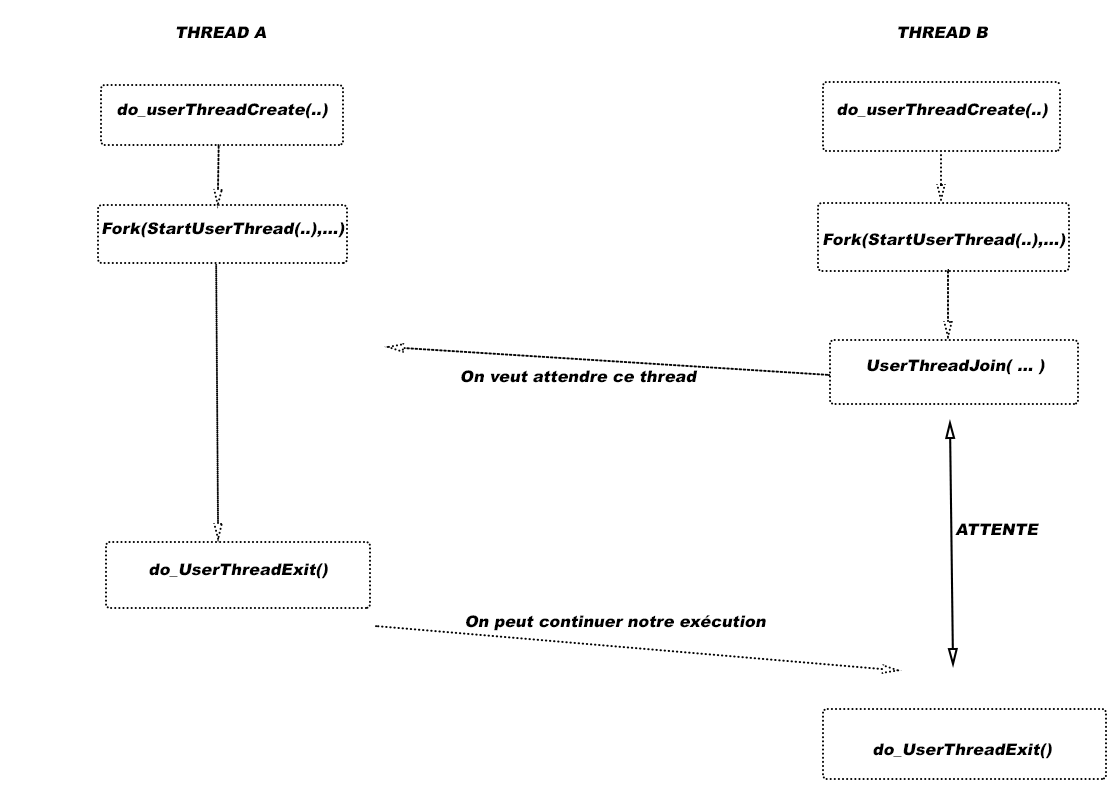
\includegraphics[scale=0.39]{./nachos_join.png}
   \caption{\label{join} Déroulemet de l'exécution}
  \end{center}
\end{figure}

On peut par ailleurs noter que cette exécution est englobé dans un thread principal, comme l'a montré notre trace d'exécution.
\end{document}
